% !TEX root = GRE-Textbook.tex

\documentclass[openany]{tufte-book}

\usepackage{amsfonts, amsmath, amsthm, amssymb}
\usepackage{adjustbox, caption, enumerate, fancyhdr, float, graphicx, hyperref, mathtools, minitoc, multicol, tasks, thmtools, tikz, titlesec, venndiagram, xcolor}
\usepackage[table]{xcolor}
%\usepackage{sectsty}
\usepackage[framemethod=TikZ]{mdframed}

\definecolor{fsblue}{RGB}{132,175,230}
\declaretheoremstyle[  % Blue theorem boxes
	headfont=\bfseries\color{fsblue!60!black},
	bodyfont=\normalfont,
	mdframed={
     	linewidth=2pt,
     	rightline=false, topline=false, bottomline=false,
     	linecolor=fsblue, backgroundcolor=fsblue!10,
    }]{thmblue}
    
\declaretheoremstyle[  % Blue lemma/corollary boxes
	headfont=\bfseries\color{fsblue!60!black},
	bodyfont=\normalfont,
	mdframed={
        	linewidth=2pt,
        	rightline=false, topline=false, bottomline=false,
        	linecolor=fsblue,
    }]{lemblue}
    
\declaretheoremstyle[  % Blue proofs
	headfont=\itshape\color{fsblue!60!black},
	notefont = \itshape ,
	name = Proof,
	numbered = no,
	bodyfont=\normalfont,
	qed = \qedsymbol,
	mdframed={
        	linewidth=2pt,
        	rightline=false, topline=false, bottomline=false,
        	linecolor=fsblue,
    }]{pfblue}
    
\declaretheoremstyle[  % Box for definitions
	headfont=\bfseries,
	bodyfont=\normalfont,
	numbered=no,
	mdframed={
        	linewidth=1.5pt,
        	rightline=false, topline=false, bottomline=false,
    }]{defbox}
    
\declaretheoremstyle[  % Box for problems
	headfont=\bfseries,
	bodyfont=\normalfont,
	mdframed={
        	linewidth=1.5pt,
        	rightline=false, topline=false, bottomline=false,
    }]{probbox}

\newenvironment{multienum}[1]{\begin{multicols}{#1} \begin{enumerate}[$i$.)]}{\end{enumerate}\end{multicols}}

% asmthm Environments
\theoremstyle{plain}
\declaretheorem[style=thmblue, parent=chapter]{theorem}  % Theorems
\declaretheorem[style=thmblue, sibling=theorem]{proposition}  % Propositions
\declaretheorem[style=lemblue, parent=theorem]{lemma}  % Lemmas
\declaretheorem[style=lemblue, parent=theorem]{corollary}  % Corollaries

\theoremstyle{definition}
\declaretheorem[style=defbox]{definition}  % Definitions
\declaretheorem[numbered=no]{example}  % Examples
\declaretheorem[style=probbox]{problem}  % Problems
\declaretheorem[numbered=no]{remark}  % Remarks
\newenvironment{prob}[1]  % Problem with custom number
  {\renewcommand\theproblem{#1}\problem} {\endproblem}

\theoremstyle{remark}
\newtheorem{step}{Step}  % Steps
\newtheorem{case}{Case}  % Cases
\newtheorem{Rule}{Rule}  % Rules
\declaretheorem[style=pfblue]{Prooff}  % Proofs in color
	\newenvironment{Proof}[1][ ]{\vspace{-1.75em}\begin{Prooff}[#1]}{\end{Prooff}}  % Numbered proof, removes space between thm and pf box
\declaretheorem[numbered=no]{solution}  % Solutions

% Shortcuts for number systems
\newcommand{\N}{\ensuremath{\mathbb{N}}}
\newcommand{\Z}{\ensuremath{\mathbb{Z}}}
\newcommand{\Q}{\ensuremath{\mathbb{Q}}}
\newcommand{\R}{\ensuremath{\mathbb{R}}}
\newcommand{\C}{\ensuremath{\mathbb{C}}}

% Operators
\DeclareMathOperator{\Ker}{Ker}  % Kernel
\DeclareMathOperator{\dom}{dom}  % Domain
\DeclareMathOperator{\Arg}{Arg}  % Principal argument of complex num
\DeclareMathOperator{\Log}{Log}  % Complex logarithm
\DeclareMathOperator{\conv}{conv}  % Convex hull
\DeclareMathOperator{\Hom}{Hom}  % Morphisms

\newcommand{\be}{\mathbf{e}}
\newcommand{\mcA}{\mathcal{A}}
\newcommand{\mcE}{\mathcal{E}}
\newcommand{\mcM}{\mathcal{M}}
\newcommand{\mcR}{\mathcal{R}}
\newcommand{\borR}{\mathcal{B}_\R}
\newcommand{\empt}{\varnothing}
\newcommand{\llra}{\longleftrightarrow}


% Avoids widows and orphans
\clubpenalty = 10000
\widowpenalty = 10000
\displaywidowpenalty = 10000


\hypersetup{colorlinks}% uncomment this line if you prefer colored hyperlinks (e.g., for onscreen viewing)

\fancypagestyle{plain}{}

%% Defines a subtitle command
\makeatletter
\newcommand{\plainsubtitle}{}%     plain-text-only subtitle
\newcommand{\subtitle}[1]{%
  \gdef\@subtitle{#1}%
  \renewcommand{\plainsubtitle}{#1}% use provided plain-text title
  \ifthenelse{\isundefined{\hypersetup}}%
    {}% hyperref is not loaded; do nothing
    {\hypersetup{pdftitle={\plaintitle: \plainsubtitle{}}}}% set the PDF metadata title
}

%% Makes title page resemble Tufte's VE instead of default
\renewcommand{\maketitlepage}{%
  {%
  \begin{fullwidth}%
  \fontsize{20}{20}\selectfont\par\noindent\textcolor{darkgray}{\thanklessauthor}%
  \vspace{11.5pc}%
  \fontsize{35}{40}\selectfont\par\noindent\textcolor{darkgray}{\thanklesstitle}%
  \fontsize{20}{40}\selectfont\par\noindent\textcolor{darkgray}{\plainsubtitle}%
  \vfill
  \fontsize{14}{16}\selectfont\par\noindent\thanklesspublisher%
  \end{fullwidth}%
  }%
  \thispagestyle{empty}%
}

%% Makes TOC resemble Tufte's VDQI instead of default
\titlecontents{part}%
    [0pt]% distance from left margin
    {\addvspace{0.25\baselineskip}}% above (global formatting of entry)
    {\allcaps{Part~\thecontentslabel}\allcaps}% before w/ label (label = ``Part I'')
    {\allcaps{Part~\thecontentslabel}\allcaps}% before w/o label
    {}% filler and page (leaders and page num)
    [\vspace*{0.5\baselineskip}]% after
\titlecontents{chapter}%
    [4em]% distance from left margin
    {}% above (global formatting of entry)
    {\contentslabel{2em}\large}% before w/ label (label = ``Chapter 1'')
    {\hspace{0em}\large}% before w/o label
    {\dotfill\thecontentspage}% filler and page (leaders and page num)
    [\vspace*{0.25\baselineskip}]% after
\titlecontents{section}%
    [8em]% distance from left margin
    {}% above (global formatting of entry)
    {\contentslabel{3em}\textit}% before w/ label (label = ``Section 1.1'')
    {\hspace{0em}\textit}% before w/o label
    {\qquad\thecontentspage}% filler and page (leaders and page num)
    [\vspace*{0.25\baselineskip}]% after

%%
% If they're installed, use Bergamo and Chantilly from www.fontsite.com.
% They're clones of Bembo and Gill Sans, respectively.
\IfFileExists{bergamo.sty}{\usepackage[osf]{bergamo}}{}% Bembo
\IfFileExists{chantill.sty}{\usepackage{chantill}}{}% Gill Sans

%\usepackage{microtype}

% Just some sample text
\usepackage{lipsum}

% For nicely typeset tabular material
\usepackage{booktabs}

% For graphics / images
\usepackage{graphicx}
\setkeys{Gin}{width=\linewidth,totalheight=\textheight,keepaspectratio}
\graphicspath{{graphics/}}

% The fancyvrb package lets us customize the formatting of verbatim
% environments.  We use a slightly smaller font.
\usepackage{fancyvrb}
\fvset{fontsize=\normalsize}

% Prints argument within hanging parentheses (i.e., parentheses that take
% up no horizontal space).  Useful in tabular environments.
\newcommand{\hangp}[1]{\makebox[0pt][r]{(}#1\makebox[0pt][l]{)}}

% Prints an asterisk that takes up no horizontal space.
% Useful in tabular environments.
\newcommand{\hangstar}{\makebox[0pt][l]{*}}

% Prints a trailing space in a smart way.
\usepackage{xspace}

% Inserts a blank page
\newcommand{\blankpage}{\newpage\hbox{}\thispagestyle{empty}\newpage}

\usepackage{units}

% Typesets the font size, leading, and measure in the form of 10/12x26 pc.
\newcommand{\measure}[3]{#1/#2$\times$\unit[#3]{pc}}

% Macros for typesetting the documentation
\newcommand{\hlred}[1]{\textcolor{Maroon}{#1}}% prints in red
\newcommand{\hangleft}[1]{\makebox[0pt][r]{#1}}
\newcommand{\hairsp}{\hspace{1pt}}% hair space
\newcommand{\hquad}{\hskip0.5em\relax}% half quad space
\newcommand{\TODO}{\textcolor{red}{\bf TODO!}\xspace}
\newcommand{\ie}{\textit{i.\hairsp{}e.}\xspace}
\newcommand{\eg}{\textit{e.\hairsp{}g.}\xspace}
\newcommand{\na}{\quad--}% used in tables for N/A cells
\providecommand{\XeLaTeX}{X\lower.5ex\hbox{\kern-0.15em\reflectbox{E}}\kern-0.1em\LaTeX}
\newcommand{\tXeLaTeX}{\XeLaTeX\index{XeLaTeX@\protect\XeLaTeX}}
% \index{\texttt{\textbackslash xyz}@\hangleft{\texttt{\textbackslash}}\texttt{xyz}}
\newcommand{\tuftebs}{\symbol{'134}}% a backslash in tt type in OT1/T1
\newcommand{\doccmdnoindex}[2][]{\texttt{\tuftebs#2}}% command name -- adds backslash automatically (and doesn't add cmd to the index)
\newcommand{\doccmddef}[2][]{%
  \hlred{\texttt{\tuftebs#2}}\label{cmd:#2}%
  \ifthenelse{\isempty{#1}}%
    {% add the command to the index
      \index{#2 command@\protect\hangleft{\texttt{\tuftebs}}\texttt{#2}}% command name
    }%
    {% add the command and package to the index
      \index{#2 command@\protect\hangleft{\texttt{\tuftebs}}\texttt{#2} (\texttt{#1} package)}% command name
      \index{#1 package@\texttt{#1} package}\index{packages!#1@\texttt{#1}}% package name
    }%
}% command name -- adds backslash automatically
\newcommand{\doccmd}[2][]{%
  \texttt{\tuftebs#2}%
  \ifthenelse{\isempty{#1}}%
    {% add the command to the index
      \index{#2 command@\protect\hangleft{\texttt{\tuftebs}}\texttt{#2}}% command name
    }%
    {% add the command and package to the index
      \index{#2 command@\protect\hangleft{\texttt{\tuftebs}}\texttt{#2} (\texttt{#1} package)}% command name
      \index{#1 package@\texttt{#1} package}\index{packages!#1@\texttt{#1}}% package name
    }%
}% command name -- adds backslash automatically
\newcommand{\docopt}[1]{\ensuremath{\langle}\textrm{\textit{#1}}\ensuremath{\rangle}}% optional command argument
\newcommand{\docarg}[1]{\textrm{\textit{#1}}}% (required) command argument
\newenvironment{docspec}{\begin{quotation}\ttfamily\parskip0pt\parindent0pt\ignorespaces}{\end{quotation}}% command specification environment
\newcommand{\docenv}[1]{\texttt{#1}\index{#1 environment@\texttt{#1} environment}\index{environments!#1@\texttt{#1}}}% environment name
\newcommand{\docenvdef}[1]{\hlred{\texttt{#1}}\label{env:#1}\index{#1 environment@\texttt{#1} environment}\index{environments!#1@\texttt{#1}}}% environment name
\newcommand{\docpkg}[1]{\texttt{#1}\index{#1 package@\texttt{#1} package}\index{packages!#1@\texttt{#1}}}% package name
\newcommand{\doccls}[1]{\texttt{#1}}% document class name
\newcommand{\docclsopt}[1]{\texttt{#1}\index{#1 class option@\texttt{#1} class option}\index{class options!#1@\texttt{#1}}}% document class option name
\newcommand{\docclsoptdef}[1]{\hlred{\texttt{#1}}\label{clsopt:#1}\index{#1 class option@\texttt{#1} class option}\index{class options!#1@\texttt{#1}}}% document class option name defined
\newcommand{\docmsg}[2]{\bigskip\begin{fullwidth}\noindent\ttfamily#1\end{fullwidth}\medskip\par\noindent#2}
\newcommand{\docfilehook}[2]{\texttt{#1}\index{file hooks!#2}\index{#1@\texttt{#1}}}
\newcommand{\doccounter}[1]{\texttt{#1}\index{#1 counter@\texttt{#1} counter}}

% Generates the index
\usepackage{makeidx}
\makeindex

% Metadata
\title{Fundamentals of Mathematics}
\subtitle{for the GRE Quantitative Reasoning Section}
\author{\itshape Carson Mitchell}
\publisher{}

\setcounter{secnumdepth}{3}

\begin{document}

\frontmatter
\maketitle
\blankpage

\setcounter{tocdepth}{1}
\tableofcontents
\listoffigures
\listoftables
\listoftheorems

\chapter{Introduction}
    % Assumption about knowing how to add multiply divide and subtract

\mainmatter
\part{Preliminaries}\label{pt:prelim}

    \chapter{Logic}\label{ch:logic}

    \section{Propositional Logic}\label{sec:proplog}
        \begin{definition}[Proposition]\label{def:prop}\index{proposition}
            A \textbf{proposition} is a statement that is either true or false.
        \end{definition}

        We often denote propositions with letters like $p,q$, or $r$. Further, we denote the truth value of a proposition with $T$ or $F$ to indicate the proposition is true or false, respectively. The area of logic that deals with propositions is \textbf{propositional logic}\index{propositional logic}. We often examine more complicated propositions, called \textbf{compound propositions}, that are formed from existing propositions using logical operators\index{logical operators}.

        There is one unary logical operator, i.e., a logical operator that applies to exactly one proposition to create a new proposition.

        \begin{definition}[Negation]\label{def:neg}\index{logical operators!negation}
            The \textbf{negation} of a proposition $p$ is $\neg p$, which is the proposition "not $p$".
        \end{definition}

        This operator negates the truth value of $p$, meaning $\neg p = T$ precisely when $p=F$, and $\neg p = F$ when $p=T$.

        \newthought{When an operator} applies to at least two propositions, it is a \textbf{connective}\index{logical operators!connectives}, and forms what is known as a \textbf{compound proposition}\index{compound propositions}.
        
        \begin{definition}[Disjunction]\label{def:disj}\index{logical operators!connectives!disjunction}
            The \textbf{disjunction} of propositions $p$ and $q$ is $p \lor q$, which is the proposition "$p$ or $q$".
        \end{definition}

        The disjunction of $p$ and $q$ is true when at least one of $p$ and $q$ are true, possibly both. It is false precisely when both $p$ and $q$ are false. 
        
        \begin{definition}[Conjunction]\label{def:conj}\index{logical operators!connectives!conjunction}
            The \textbf{conjunction} of propositions $p$ and $q$ is $p \land q$, which is the proposition "$p$ and $q$".
        \end{definition}

        The conjunction of $p$ and $q$ is true precisely when $p$ and $q$ are \emph{both} true, and false otherwise.\sidenote{The conjunction can be thought of as "both $p$ is true \emph{and} $q$ is true".} In the case where we want to represent the proposition "exactly one of $p$ and $q$ is true, but not both", we can use the \textbf{exclusive-or}\index{logical operators!connectives!exclusive-or}, denoted by $p \oplus q$. The exclusive-or is false exactly when $p$ and $q$ take the same truth value, true otherwise.

        \newthought{A visual tool} that can be helpful for understanding the conditions under which a given compound proposition is true, based on the truth values of its constituent propositions, is a \textbf{truth table}\index{truth tables}. A truth table is an array that highlights all possible combinations of constituent propositions' truth values.

        \begin{example}[Truth Table for a Conjunction]\label{ex:conjtt}
            The truth table for the conjunction $p \land q$ is:
            \begin{table}[h]
    \centering
    \begin{tabular}{|c|c||c|}
        \hline $\mathbf{p}$ & $\mathbf{q}$ & $\mathbf{p \land q}$ \\
        \hline \cellcolor{green!25}$T$ & \cellcolor{green!25}$T$ & \cellcolor{green!25}$T$ \\
        \hline \cellcolor{green!25}$T$ & \cellcolor{red!25}$F$ & \cellcolor{red!25}$F$ \\
        \hline \cellcolor{red!25}$F$ & \cellcolor{green!25}$T$ & \cellcolor{red!25}$F$ \\
        \hline \cellcolor{red!25}$F$ & \cellcolor{red!25}$F$ & \cellcolor{red!25}$F$ \\
        \hline
    \end{tabular}
        \caption{The truth table for $p \land q$.}
        \label{tab:conjtab}
\end{table}
            
            \noindent and we can observe that the four possible combinations for the simultaneous truth values of $p$ and $q$ are included in the rows left of the double vertical line. The truth values for $p \land q$ on the right correspond to the combination of values for $p$ and $q$ in their respective row. \qed
        \end{example}
        
        \newthought{The next type of connective} is named the \textbf{conditional operator} or \textbf{implication}.

        \begin{definition}[Implication]\label{def:imp}\index{logical operators!connectives!implication}
            Given propositions $p$ and $q$, the \textbf{implication} $p \rightarrow q$ is the proposition "if $p$, then $q$".
        \end{definition}

        The implication $p \to q$ is false exactly when $p$ is false and $q$ is true, and true otherwise. We call the proposition $p$ the \textbf{antecedent} or \textbf{premise}, and the proposition $q$ the \textbf{consequent} or \textbf{conclusion}.
        
        It is important to note that a logical implication need not depend on our intuition of causation to be true. For example, $p \to q$ is true when both $p$ and $q$ are true; so, if $p$ is the proposition "the author's name is Carson" and $q$ is the proposition "$2+2=4$", then $p \to q$ ("If the author's name is Carson, then $2+2=4$") is true. This, however, does not necessarily mean that the author's name being Carson causes $2+2=4$ to be true.

        Further, it can cause some confusion to understand that $p \to q$ is true whenever $p$ is false. Consider the following example to illustrate. Let $p$ be the proposition "unicorns are real". In this case, regardless of what $q$ is, we say that $p \to q$ is true because, in a universe where unicorns are real, it's not outside the realm of possibility that whatever $q$ claims is also true, as we have no legitimate insight into what such a universe may look like or consist of.

        The implication has some relatives, one of which is logically equivalent, a topic we will discuss in greater detail momentarily. The \textbf{converse}\label{def:conv}\index{logical operators!connectives!converse} of the implication $p \to q$ is the proposition $q \to p$. The \textbf{inverse}\label{def:inv}\index{logical operators!connectives!inverse} of the implication $p \to q$ is the proposition $(\neg p) \to (\neg q)$. Note that the converse switches the order of the antecedent and consequent, while the inverse negates each, respectively, but does not switch the order. 

        \begin{definition}[Contrapositive]\label{def:contrapos}\index{logical operators!connectives!contrapositive}
            The \textbf{contrapositive} of the implication $p \to q$ is the proposition $(\neg q) \to (\neg p)$.
        \end{definition}

        The contrapositive, as we will prove, is entirely equivalent to the original implication. Meaning, the truth value of one is \emph{always} the same as the truth value of the other. Finally, we introduce the last major logical connective.

        \begin{definition}[Biconditional]\label{def:bicon}\index{logical operators!connectives!biconditional}
            The \textbf{biconditional} of propositions $p$ and $q$ is the proposition $(p \to q) \land (q \to p)$, denoted $p \longleftrightarrow q$ and read as "$p$ if and only if $q$". 
        \end{definition}
        
        We can observe that $p \longleftrightarrow q$ is true exactly when $p$ and $q$ take on the same truth value, false otherwise\sidenote{$p \longleftrightarrow q$ is false exactly when $p \oplus q$ is true; i.e. $p \llra q$ is equivalent to $\neg (p \oplus q)$.}. This should indicate to the reader that, in a sense, $p$ and $q$ are equivalent when $p \longleftrightarrow q$ is a true proposition.
        
        As a note on English translations\sidenote{Oftentimes, you may see authors abbreviate the phrase "if and only if" as "iff".}, some phrases that often give students trouble are "$p$ if $q$" and "$p$ only if $q$". The former is equivalent to the implication $q \to p$ while the latter is equivalent to the implication $p \to q$. Thus, if we see the phrase "if and only if", we can recognize we are working with a biconditional. 

        \newthought{Given the implication} $p \to q$, we say that $p$ is a \textbf{sufficient} condition for $q$, and $q$ is a \textbf{necessary} condition for $p$. We say $p$ is sufficient because $p$ being true is "enough" to assure that $q$ is true, but it's possible there are other conditions besides $p$ that would also satisfy $q$. Similarly, we say $q$ is necessary because, for $p$ to be true, it is required that $q$ be true.

        We now note that there exists an order in which logical operators are executed. It is best practice to always use parentheses, as used previously, to indicate smaller atomic parts within a compound proposition. Contents within parentheses are always evaluated first; then, the negation operator applies to the proposition most right-adjacent to it; then, the conjunction and disjunction operators are applied; then, the implication; finally, the biconditional.

        Below, for reference, are included truth tables containing all of the compound propositions covered thus far, as well as the implication and its various related forms.

        \begin{table}[h]
    \centering
    \begin{tabular}{|c|c||c|c|c|c|c|}
        \hline $\mathbf{p}$ & $\mathbf{q}$ & $\mathbf{p \land q}$ & $\mathbf{p \lor q}$ & $\mathbf{p \oplus q}$ & $\mathbf{p \to q}$ & $\mathbf{p \longleftrightarrow q}$ \\
        \hline \cellcolor{green!25}$T$ & \cellcolor{green!25}$T$ & \cellcolor{green!25}$T$ & \cellcolor{green!25}$T$ & \cellcolor{red!25}$F$ & \cellcolor{green!25}$T$ & \cellcolor{green!25}$T$ \\
        \hline \cellcolor{green!25}$T$ & \cellcolor{red!25}$F$ & \cellcolor{red!25}$F$ & \cellcolor{green!25}$T$ & \cellcolor{green!25}$T$ & \cellcolor{red!25}$F$ & \cellcolor{red!25}$F$ \\
        \hline \cellcolor{red!25}$F$ & \cellcolor{green!25}$T$ & \cellcolor{red!25}$F$ & \cellcolor{green!25}$T$ & \cellcolor{green!25}$T$ & \cellcolor{green!25}$T$ & \cellcolor{red!25}$F$ \\
        \hline \cellcolor{red!25}$F$ & \cellcolor{red!25}$F$ & \cellcolor{red!25}$F$ & \cellcolor{red!25}$F$ & \cellcolor{red!25}$F$ & \cellcolor{green!25}$T$ & \cellcolor{green!25}$T$ \\
        \hline
    \end{tabular}
        \caption{Truth table for compound propositions involving atomic propositions $p$ and $q$.}
        \label{tab:comptab}
\end{table}
        \begin{table}[h]
    \centering
    \begin{tabular}{|c|c||c|c|c|c|c|c|}
        \hline $\mathbf{p}$ & $\mathbf{q}$ & $\mathbf{\neg p}$ & $\mathbf{\neg q}$ & $\mathbf{p \to q}$ & $\mathbf{(\neg q) \to (\neg p)}$ & $\mathbf{q \to p}$ & $\mathbf{(\neg p) \to (\neg q)}$ \\
        \hline \cellcolor{green!25}$T$ & \cellcolor{green!25}$T$ & \cellcolor{red!25}$F$ & \cellcolor{red!25}$F$ & \cellcolor{green!25}$T$ & \cellcolor{green!25}$T$ & \cellcolor{green!25}$T$ & \cellcolor{green!25}$T$ \\
        \hline \cellcolor{green!25}$T$ & \cellcolor{red!25}$F$ & \cellcolor{red!25}$F$ & \cellcolor{green!25}$T$ & \cellcolor{red!25}$F$ & \cellcolor{red!25}$F$ & \cellcolor{green!25}$T$ & \cellcolor{green!25}$T$ \\
        \hline \cellcolor{red!25}$F$ & \cellcolor{green!25}$T$ & \cellcolor{green!25}$T$ & \cellcolor{red!25}$F$ & \cellcolor{green!25}$T$ & \cellcolor{green!25}$T$ & \cellcolor{red!25}$F$ & \cellcolor{red!25}$F$ \\
        \hline \cellcolor{red!25}$F$ & \cellcolor{red!25}$F$ & \cellcolor{green!25}$T$ & \cellcolor{green!25}$T$ & \cellcolor{green!25}$T$ & \cellcolor{green!25}$T$ & \cellcolor{green!25}$T$ & \cellcolor{green!25}$T$ \\
        \hline
    \end{tabular}
        \caption{Truth table for implications of atomic propositions $p$ and $q$ and its relatives.}
        \label{tab:imptab}
\end{table}

        \newthought{We now define} a few types of categories with respect to compound propositions. A compound proposition falls into exactly one of three categories:

        \begin{definition}[Tautology]\label{def:tautology}\index{compound propositions!tautology}
            A compound proposition $P$ is a \textbf{tautology} if $P$ is always true, i.e. there is no circumstance under which the truth table of $P$ contains a false $F$ entry.
        \end{definition}
        
        \begin{definition}[Contradiction]\label{def:contradiction}\index{compound propositions!contradiction}
            A compound proposition $P$ is a \textbf{contradiction} if $P$ is always false, i.e. there is no circumstance under which the truth table of $P$ contains a true $T$ entry.
        \end{definition}

        Any statement that could be true or false depending on the truth values of its atomic components is called a \textbf{contingency}; thus, a contingency is any compound proposition that is neither a tautology nor contradiction. We say that $P$ is \textbf{satisfiable} when it is either a tautology or contingency; i.e., there is some arrangement of the atomic constituents of $P$ that makes $P$ a true proposition; there is an instance where $P$ is not false. Further, $P$ is \textbf{unsatisfiable} when $P$ is a contradiction or, equivalently, $(\neg P)$ is a tautology. An assignment of truth values to the atomic constituents of a satisfiable $P$ that makes $P$ true is called a \textbf{solution}.

        \newthought{We may now formally define} what it means for two propositions to be equivalent in logic.

        \begin{definition}[Logical Equivalence]\label{def:logeq}\index{logical equivalence}
            Compound propositions $P$ and $Q$ are \textbf{logically equivalent}, denoted $P \equiv Q$, when $P \longleftrightarrow Q$ is a tautology.
        \end{definition}

        In other words, $P \equiv Q$ when they share the same truth table (always take on the same truth value). Equivalent forms hold great importance in logic because they allow for one compound proposition to be substituted for another at any point, which enables different modes of understanding or proving a given proposition, oftentimes to the benefit of simplicity or intuition. Below we share some equivalences involving a single compound proposition.  

        \begin{theorem}[Equivalent Logical Forms]\label{thm:eqlogforms}
            The following hold:
            \begin{enumerate}
                \item \textbf{Identity:} $P \land T \equiv P$ and $P \lor F \equiv P$.
                \item \textbf{Domination:} $P \lor T \equiv T$ and $P \land F \equiv F$.
                \item \textbf{Idempotence:} $P \lor P \equiv P$ and $P \land P \equiv P$.
                \item \textbf{Double Negation:} $\neg(\neg P) \equiv P$.
                \item \textbf{Negation Operations:} $P \lor (\neg P) \equiv T$ and $P \land (\neg P) \equiv F$.
            \end{enumerate}
        \end{theorem}

        Now, we share some equivalences involving two or more compound propositions.

        \begin{theorem}[Equivalent Logical Forms II]\label{thm:eqlogforms2}
            The following hold:
            \begin{enumerate}
                 \item \textbf{Commutativity:} $P \lor Q \equiv Q \lor P$ and $P \land Q \equiv Q \land P$.
                \item \textbf{Absorption:} $P \lor (P \land Q) \equiv P$ and $P \land (P \lor Q) \equiv P$.
                \item \textbf{DeMorgan's Laws:} $$\neg(P \lor Q) \equiv (\neg P) \land (\neg Q)$$ $$\neg(P \land Q) \equiv (\neg P) \lor (\neg Q)$$
                \item \textbf{Associativity:} $$(P \lor Q) \lor R \equiv P \lor (Q \lor R)$$ $$(P \land Q) \land R \equiv P \land (Q \land R)$$
                \item \textbf{Distributivity:} $$P \lor (Q \land R) \equiv (P \lor Q) \land (P \lor R)$$ $$P \land (Q \lor R) \equiv (P \land Q) \lor (P \land R)$$
            \end{enumerate}
        \end{theorem}

        Next, we share some equivalences involving implications.

        \begin{theorem}[Equivalent Logical Forms III]\label{thm:eqlogforms3}
            The following hold:
            \begin{enumerate}
                \item \textbf{Contraposition:} $P \to Q \equiv (\neg Q) \to (\neg P)$.
                \item \textbf{Implication-Disjunction Relationship:} $$P \lor Q \equiv (\neg P) \to Q \text{ and } P \to Q \equiv (\neg P) \lor Q.$$
                \item \textbf{Implication-Conjunction Relationship:} $$P \land Q \equiv \neg\left(P \to (\neg Q)\right) \text{ and } \neg(P \to Q) \equiv P \land (\neg Q).$$
                \item \textbf{Distributivity over Premises:} $$(P \lor Q) \to R \equiv (P \to R) \land (Q \to R)$$ $$(P \land Q) \to R \equiv (P \to R) \lor (Q \to R)$$
                \item \textbf{Distributivity over Conclusions:} $$P \to (Q \lor R) \equiv (P \to Q) \lor (P \to R)$$ $$P \to (Q \land R) \equiv (P \to Q) \land (P \to R)$$
            \end{enumerate}
        \end{theorem}

        Finally, we conclude with some equivalences involving biconditionals.

        \begin{theorem}[Equivalent Logical Forms IV]\label{thm:eqlogforms4}
            The following hold:
            \begin{enumerate}
                \item $P \longleftrightarrow Q \equiv (\neg P) \longleftrightarrow (\neg Q)$.
                \item $P \longleftrightarrow Q \equiv (P \land Q) \lor \left((\neg P) \land (\neg Q)\right) \equiv \neg(P \oplus Q)$.
                \item $P \longleftrightarrow Q \equiv \left(P \lor (\neg Q)\right) \land \left((\neg P) \lor Q\right)$.
                \item $\neg(P \longleftrightarrow Q) \equiv P \longleftrightarrow (\neg Q) \equiv (\neg P) \longleftrightarrow Q$.
                \item $\neg(P \longleftrightarrow Q) \equiv (P \lor Q) \land \left((\neg P) \lor (\neg Q)\right) \equiv P \oplus Q$.
                \item $\neg(P \longleftrightarrow Q) \equiv \left(P \land (\neg Q)\right) \lor \left((\neg P) \land Q\right)$.
            \end{enumerate}
        \end{theorem}
        

    \section{First-Order Logic}\label{sec:folog}

        \textbf{First-order logic} or \textbf{predicate logic} is an important extension of propositional logic that allows for a large expansion to the possible sentences that can be converted into symbolic form and analyzed for validity, making it an incredibly valuable tool in the assessment of arguments.

        In propositional logic, we assume that each atomic proposition ($p$, $q$, $r$, etc.) can be assessed for soundness and declared absolutely true or absolutely false. In other words, once a proposition is specified, we can with certainty decide that it is a true proposition or a false proposition. In first-order logic, we allow for our atomic statements to possess a degree of variability -- even when specified, there are cases where a statement can be true and other cases where it can be false, not possessing an intrinsic truth value. This leads to two important definitions: the qualities that define claims (\textbf{predicates}) and the extent to which the claims can be true over a specified domain (\textbf{quantifiers}). The study of these two concepts and their relationships is what comprises the foundation of first-order logic.

        \begin{definition}[Predicate]\label{def:predicate}\index{predicate}
            A \textbf{predicate} is a property that can be applied to an object/subject to produce a proposition.
        \end{definition}

        Because a predicate depends on an object to become a proposition, the combination of a predicate and unknown object is referred to as an \textbf{open proposition} or \textbf{propositional function}.

        \begin{example}[Predicate]\label{ex:predicate}
            The statement "\ldots is a city in California" is an open proposition because its truth value entirely depends on what words take the place of the ellipsis. The predicate/property here is being a city in California. It becomes a true proposition if we were to substitute "San Francisco" for the ellipsis, but a false proposition if we were to substitute "New York City" for the ellipsis.

            Instead of an ellipsis, it is commonplace to use letters like $x$, $y$, and $z$ to denote the unknown elements of an open proposition. If we say the predicate $P$ is being a city in California, then $P(x)$ can be used to denote the open proposition "$x$ is a city in California". $P(x)$ has no intrinsic truth value, but when values are substituted for $x$, we have definite propositions with truth values. $P($San Francisco$) = T$ and $P($New York City$) = F$. \qed
        \end{example}

        Open propositions with more than one variable element are commonplace. If a predicate depends on two inputs, we may write $P(x,y)$; further, for $n$ inputs, we may write $P(x_1, x_2, \ldots, x_n)$.

        %universal set

        % natural language translations (symbols will be dropped in many cases in future use)


    \section{Proofs}\label{sec:proof}
        % define theorems, lemmas, corollaries



    
    
    \chapter{Set Theory}\label{ch:set}

    \section{Sets}
        \begin{definition}[Set]\label{def:set}\index{set}
            A \textbf{set} is an \emph{unordered} collection of \emph{distinct} elements.
        \end{definition}

        Note the emphasis on the keywords \emph{unordered} \sidenote{A set has no order of elements, meaning, for example, the sets $\{a,b,c\}$ and $\{c,a,b\}$ are considered the same set.} and \emph{distinct}.\sidenote{Elements cannot be members of a set more than once; they are either a member or not a member. As an example, $\{a,a,b,c\}$ is really just the set $\{a,b,c\}$.}
        We can write out the contents of a set explicitly using brackets: e.g. $$S = \{2,4,6,8 \},$$ or by specifying some property: $$S = \{x: x \text{ is an even integer between $0$ and $10$}\},$$ read "the set of all $x$ such that $x$ is an even integer between $0$ and $10$."

        If $x$ is an element of the set $S$, we write $x \in S$; otherwise, we write $x \not\in S$. Typically, lowercase letters denote elements and uppercase letters denote sets, with some exceptions to be discussed later.

        We say two sets $A$ and $B$ are \textbf{equivalent} when they have the same elements. In other terms, $A=B$ when $\forall x(x\in A \longleftrightarrow x\in B)$. The unique set with no elements is called the \textbf{empty set}\index{set!empty set} and is denoted by the symbol $\empt$. A set with exactly one element is a \textbf{singleton}\index{set!singleton}.

        \newthought{It is a common theme in mathematics} that once an object of study is specified, smaller components of that object that constitute an object in their own right are studied as well -- especially their relationship to the larger ambient object. This begins in set theory.

        \begin{definition}[Subset]\label{def:subset}\index{set!subset}
            A set $A$ is a \textbf{subset} of a set $B$ when every element of $A$ is an element of $B$, denoted $A \subseteq B$. $$\forall x (x \in A \longrightarrow x\in B)$$
        \end{definition}

        It is vacuously true that any set $A$ is a subset of itself, $A \subseteq A$. In fact, every set has two \textbf{trivial subsets}, itself and $\empt$. We say $A$ is a \textbf{proper subset} of $B$ when $A \subseteq B$ \emph{and} there exists some element of $B$ that is not an element of $A$, denoted $A \subset B$.\sidenote{For example, $\{a,b,c\}$ is a proper subset of $\{a,b,c,d\}$.} Further, we can say $A=B$ if and only if $A \subseteq B$ \emph{and} $B \subseteq A$; in fact, this is often the method used in practice to show two sets are equivalent -- prove each set is a subset of the other.

    \section{Set Operations}\label{sec:setops}\index{set operations}
    % Universal set
        \newthought{We can perform well-defined operations} on existing sets to produce new sets.

        \begin{definition}[Union]\label{def:union}\index{set operations!union}
            The \textbf{union} of sets $A$ and $B$ is the set $$A\cup B = \left\{x\in U: (x\in A) \lor (x\in B)\right\}.$$
        \end{definition}

        \begin{marginfigure}
            \begin{venndiagram2sets}[shade=fsblue, labelA=, labelB=,    labelOnlyA=$A$, labelOnlyB=$B$, labelNotAB=$U$]
    \fillA \fillB
\end{venndiagram2sets}
            \caption{The set $A \cup B$}
            \label{fig:union}
            \setfloatalignment{t}
        \end{marginfigure}
        
        This means that $x \in A \cup B$ exactly when $x$ is a member of $A$, or a member of $B$, or potentially a member of both $A$ and $B$. 
        On the other hand, we can define:

        \begin{definition}[Intersection]\label{def:intersec}\index{set operations!intersection}
            The \textbf{intersection} of sets $A$ and $B$ is the set $$A\cap B = \left\{x\in U: (x\in A) \land (x\in B)\right\}.$$
        \end{definition}

        \begin{marginfigure}
            \begin{venndiagram2sets}[shade=fsblue, labelA=, labelB=,    labelOnlyA=$A$, labelOnlyB=$B$, labelNotAB=$U$]
    \fillACapB
\end{venndiagram2sets}
            \caption{The set $A \cap B$}
            \label{fig:intersection}
            \setfloatalignment{t}
        \end{marginfigure} 

        We have $x \in A \cap B$ if and only if $x$ is both a member of $A$ and a member of $B$. 
        
        One can readily observe that $(A \cap B) \subseteq (A \cup B)$, with $(A\cap B) = (A \cup B)$ if and only if $A=B$; otherwise, $(A \cap B) \subset (A \cup B)$. We say two sets $A$ and $B$ are \textbf{disjoint}\index{set!disjoint sets} when they share no elements in common, i.e. $A \cap B = \empt$.

        \begin{definition}[Difference]\label{def:diff}\index{set operations!set difference}
            The \textbf{difference} of sets $A$ and $B$ is the set $$A - B = \left\{x\in U: (x\in A) \land (x\not\in B)\right\}.$$
        \end{definition}

        \begin{marginfigure}
            \begin{venndiagram2sets}[shade=fsblue, labelA=, labelB=,    labelOnlyA=$A$, labelOnlyB=$B$, labelNotAB=$U$]
    \fillANotB
\end{venndiagram2sets}
            \caption{The set $A - B$}
            \label{fig:difference}
            \setfloatalignment{t}
        \end{marginfigure}

        This represents the set $A$ with everything shared in common with $B$ removed. This implies $(A - B) \cap B = \empt$ and $(A-B) \subseteq A$, with equality when $A$ and $B$ are disjoint.

        \begin{definition}[Complement]\label{def:comp}\index{set operations!complement}
            The \textbf{complement} of a set $A$ with respect to its ambient universe $U$ is the set $$A^c = \left\{x\in U: x\not\in A\right\}.$$
        \end{definition}

        \begin{marginfigure}
            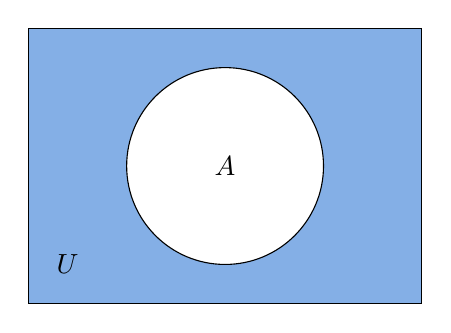
\begin{tikzpicture}
    \filldraw[fill=fsblue] (0,0) rectangle (5,3.5);
    \node at (0.5,0.5) {$U$};
    
    % Draw the single set A (circle)
    \filldraw[fill=white] (2.5,1.75) circle (1.25);
    \node at (2.5,1.75) {$A$};
\end{tikzpicture}
            \caption{The set $A^c$}
            \label{fig:complement}
            \setfloatalignment{t}
        \end{marginfigure}

        The complement of $A$ is all elements in the defined universe $U$ that are not in $A$. These definitions allow for some important properties of set operations, which can all be proven from definitions if desired; they should all be studied carefully and well-understood.

        \begin{theorem}[Set Properties]\label{thm:setprop}
            The following hold for all sets:
            \begin{enumerate}
                \item \textbf{Identity:} $A \cap U = A$ and $A \cup \empt = A$.
                \item \textbf{Domination:} $A \cup U = U$ and $A \cap \empt = \empt$.
                \item \textbf{Idempotence:} $A \cup A = A$ and $A \cap A = A$.
                \item \textbf{Double Complementation:} $(A^c)^c = A$.
                \item \textbf{Complement Operations:} $A \cup A^c = U$ and $A \cap A^c = \empt$.
                \item \textbf{Commutativity:} $A \cup B = B \cup A$ and $A \cap B = B \cap A$.
                \item \textbf{Absorption:} $A \cup (A\cap B) = A$ and $A \cap (A \cup B) = A$.
                \item \textbf{DeMorgan's Laws:} $$(A \cup B)^c = A^c \cap B^c$$ $$(A \cap B)^c = A^c \cup B^c$$
                \item \textbf{Associativity:} $$(A \cup B) \cup C = A \cup (B \cup C)$$ $$(A \cap B) \cap C = A \cap (B \cap C)$$
                \item \textbf{Distributivity:} $$A \cup (B \cap C) = (A\cup B) \cap (A \cup C)$$ $$A \cap (B \cup C) = (A\cap B) \cup (A \cap C)$$
            \end{enumerate}
        \end{theorem}

        %natural numbers definition, binary operations
        %ordering



    
\part{Arithmetic}\label{pt:arithmetic}

    \chapter{Standard Arithmetic}\label{ch:arith}

    \section{Integers}\label{sec:ints}
        Recall that the \textbf{natural numbers} are defined as
        \[\N = \{0,1,2,3,4,5,6,\ldots\}.\] 
        The binary operation of addition $+:\N^2 \to \N$ takes two \textbf{addends}, say $a$ and $b$, and outputs a \textbf{sum}, $+(a,b)$, which we denote by $a + b$. We can observe (and prove, if desired) a few important properties about this operation.

        \begin{theorem}[Properties of Addition]\label{thm:PoA}
            When defined on \N,
            \begin{enumerate}
                \item \textbf{Closure:} If $a, b \in \N$, then $a + b \in \N$.
                \item \textbf{Associativity:} For all $a,b,c \in \N$ $$(a+b)+c = a+(b+c).$$
                \item \textbf{Identity:} For all $a \in \N$ $$a+0=0+a=a.$$ We call $0$ the \textbf{additive identity} in $\N$.
                \item \textbf{Commutativity:} For all $a,b \in \N$ $$a+b=b+a.$$
                \item \textbf{Cancellation Property:} For all $a,b,c \in \N$ $$\text{if } a+c = b+c \text{, then } a = b.$$
            \end{enumerate}
        \end{theorem}

        The closure property indicates that the sum of two natural numbers is also a natural number; we call the set of natural numbers "closed" under addition. The associative property shows that, in a string of numbers added together, it need not matter which two are added together first. We can add from right to left, left to right, or start at some arbitrary point in the middle. The identity property shows the existence of an "identity" under addition (in this case $0$), where a number remains unchanged when added to the identity. The commutativity property shows that switching the order of addends has no effect on the sum.\sidenote{Using associativity and commutativity together allows for incredible flexibility in performing a long string of addition in whatever way feels most convenient or simple to us.} The cancellation law shows that if adding the same number to addends results in the same sum, the initial addends must also be the same.

        \newthought{The binary operation of} \textbf{multiplication} can be defined on the natural numbers as the act of repeated addition. We define $\cdot:\N^2 \to \N$ by:
        $$\cdot(a,b) = a\cdot b = \underbrace{a + a + \cdots + a}_{b \text{ times}}.$$ We say $a$ and $b$ are the \textbf{factors} and $ab$ is the \textbf{product}.\sidenote{We often omit the dot entirely and just express the product as $ab$.} The multiplication operation also possesses many nice properties (which can also be proven) that allow for ease of computation.

        \begin{theorem}[Properties of Multiplication]\label{thm:PoM}
            When defined on \N,
            \begin{enumerate}
                \item Multiplication is closed.
                \item Multiplication is associative.
                \item The \textbf{multiplicative identity} is $1$.
                \item Multiplication is commutative.
                \item \textbf{Cancellation Property:} For all $a,b,c \in \N$ such that $c \neq 0$ $$\text{if } ac=bc \text{, then } a=b.$$
                \item \textbf{Zero Property:} For all $a \in \N$ $$a\cdot 0 = 0 \cdot a = 0.$$
                \item \textbf{Zero Product Property:} For all $a,b \in \N$ $$\text{if } ab=0 \text{, then } a=0 \text{ or } b=0.$$
                \item \textbf{Distributivity:} For all $a,b,c \in \N$ $$a(b+c) = ab + ac.$$
            \end{enumerate}
        \end{theorem}


    \section{Rational Numbers}\label{sec:rats}
    
    \chapter{Number Theory}\label{ch:num}

\part{Algebra}\label{pt:alg}

\part{Geometry}\label{pt:geo}

    \chapter{Circles}\label{ch:circles}

    \chapter{Trigonometry}\label{ch:trig}

\part{Data Analysis}\label{pt:data}

    \chapter{Combinatorics}\label{ch:combo}

    \chapter{Discrete Probability}\label{ch:prob}

\part*{Bibliography and Index}
\backmatter
\bibliography{sample-handout}
\bibliographystyle{plainnat}
\printindex

\end{document}